% ====================
\chapter{Back-in Parking for Powered Wheelchairs}
\label{ch:wheelchair}
% ====================

We validate the viability of the algorithm by implementing a back-in parking
system for a powered wheelchair.

% ===================================================
\section{Hardware}
% ===================================================

[TODO photo]

We choose and fix the hardware used beforehand.

We use an RGB-D sensor due to its suitability to the problem:
it works well indoors, where the target users will be using the wheelchairs; it
is cost effective; it provides depth information with adequate accuracy.

We use only one camera. This is for simplicity. Each camera saturates its USB
controller, hence a computer must have as many USB controllers as cameras.
An additional calibration step to register the information, increasing the
computational costs even further than the linear factor. 
One can argue a limitation of using one RGB-D sensor is the depth measurements
have a range of around 0.6 m to 8 m, with a field of view of 43 degrees
vertically by 57 degrees horizontally (TODO better reference) \cite{endres2014catadioptric},
comparatively limited to lidars with fields of view of 180 degrees. Some work
\cite{endres2014catadioptric} has been done using two mirrors to split the field
of view of a single camera to cover both the front and rear view. Our work
sticks to a single camera for simplicity, though it can be naturally extended.

We mount the RGB-D camera downwards. However, we do not rely on a specific angle
to keep the solutions generalizable to systems that might have different camera
angles. The only assumption is the ground plane is visible.

We use an Asus RGB-D camera as it is smaller and less obtrusive than the Kinect
and does not require an additional power plug; it gets its power entirely from
USB.


We use a (TODO model) by (TODO) 

We use a Lenovo W530 laptop with 
\begin{itemize}
\item Intel Core i7-3720QM Processor
\item 8GB RAM
\item 120GB SSD
\item NVIDIA Quadro K1000M Graphical Processing Unit
\item Two dedicated USB controllers for USB 2.0 and USB 3.0
\item Ubuntu 14.04 64-bit
\item Robotic Operating System (Indigo release)
\end{itemize}


% ====================
\section{Generating Environment Maps from RGBD Sensors}
% ====================

[TODO clean up]
We formulate the problem by creating a belief over the state space
that characterizes the desirability of the state as a parking spot.
TODO reinforcement learning terminology.

\begin{figure}
\centering
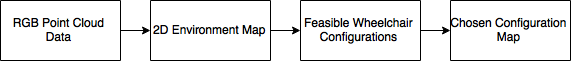
\includegraphics[width=3in]{figures/rgbdmap.png}
\caption{(TODO larger image) Pipeline for choosing a suitable parking spot.
The transition from point cloud data to a 2D environment map is described in
\autoref{sec:processingPointCloud} and \autoref{sec:2dmap}. Generating feasible configurations from the
environment map is described in \autoref{sec:feasibleparkingspot}. Selecting one
of the feasible configurations is described in
\autoref{sec:choosingparkingspot}.}
\label{fig:rgbdmap}
\end{figure}

\autoref{fig:rgbdmap} shows the general pipeline of the approach taken. The
point cloud data is transformed into a 2D environment map consisting of objects,
ground (free space), and unknown space. From this, the set of feasible
wheelchair configurations are determined, and a heuristic-based desirability
function is applied to choose an appropriate configuration from the feasible set.





% ====================
\subsection{Preprocessing the Point Cloud}
\label{sec:processingPointCloud}
% ====================
To make a map, we are inspired by the approaches of Holz \cite{holz2013towards}
and Gritti \cite{gritti2014kinect} to detect obstacles based on their height
from the ground plane. This allows detection of obstacles regardless of
their shape.

% One may argue: why not go directly from RGB-D sensor data to classification of
% parking spots, instead of a pipeline approach?
% First, we will see that ground detection is fairly robust and computationally
% cheap: there is very little error in this preprocessing step.
% Second, RGB-D data varies quite a bit; there is no clear mapping from RGB-D
% point clouds to location of parking spots. A learning approach would require an
% overbearing amount of training examples.

First, the point cloud is downsampled using a voxelized grid approach with a 5 cm
grid filter. This reduces the computational load and prevents excess weighting of
certain volumes in the upcoming ground plane detection.
Next, we estimate the parameters of a ground plane. 
The ground plane is needed for two reasons: it allows a 2D map to be easily
created aligned to the ground plane (\autoref{sec:2dmap}), and allows an
obstacle to be characterized by points above a certain distance above
the ground plane.
Multiple methods exist, including RANSAC \cite{fischler1981random}, the Hough
transform, and M-estimators \cite{holz2013towards}. We use a modified version
of RANSAC. 

Ground plane detection is done on each frame independently for robustness to
changing angles of the camera.
Algorithm \autoref{alg:modifiedRansac} shows the modified version of RANSAC.
Which ingests a point cloud $P$ of $n$ points in $\mathbb{R}^3$, and three
parameters: $k$, the number of iterations of testing a a new plane, $t$, the
threshold in metres in which points are considered part of the plane, and
$\theta_{max}$, the maximum inclination angle of possible ground planes.
Point cloud $P$ follows the format of a point cloud from an RGBD camera acquired
using the `openni2\_camera' package in ROS. This means the positive y-axis is
pointed roughly upwards in world coordinates, with the positive z-axis pointing
away from the camera along the horizontal plane of the camera.

The result is a ground plane represented as a 4-tuple $(a,b,c,d)$ satisfying
$ax + by + cz + d = 0$. Lines 7-9 highlight the additional constraint to avoid
detecting vertical planar surfaces (i.e. walls). Lines 16-18 ensure the ground
plane has a normal vector pointing upwards in the world space, standardizing any
ambiguity in defining a plane.

\begin{algorithm}
\caption{Modified RANSAC}
\label{alg:modifiedRansac}
\begin{algorithmic}[1]
\Require{
$k$ is the number of iterations to run, P are points in $\mathbb{R}^3$ with the
positive $y$ axis roughly vertical upwards, $\theta_{max}$ is the maximum
inclination angle, $t$ is the threshold used to identify if a point fits the
plane}
\Statex
\Function{ModifiedRANSAC}{$k, P, \theta_{max}, t$}
    \State $n \gets 3$, the minimum number of points to specify a plane
    \State $d \gets 0$, the number of points that lie on the current best plane
    \For{$k$ iterations}
        \State Draw a sample of $n$ non-collinear points from $P$ uniformly at random
        \State $l \gets$ the plane that includes all $n$ points
        \If{the angle between the x-z axis and plane $l$ is greater than $\theta_{max}$}
            \State the plane is too steep, continue to the next iteration
        \EndIf
        \State Find the subset of points $p \in P$ such that all points in $p$ are
        within distance $t$ from plane $l$
        \If{$|p| > d$}
            \State $bestPlane \gets l$, the current best ground plane candidate.
            \State $d \gets |p|$
        \EndIf
    \EndFor
    \If{the vector normal to $bestPlane$ has a negative $y$ coeficcient}
        \State flip the sign of the $y$ coefficient of $bestPlane$ 
    \EndIf
\EndFunction
\Statex
\Ensure{$bestPlane$, a 4-tuple $(a,b,c,d)$ that satisfies $ax + by + cz + d =
0$ representing the ground plane}
\end{algorithmic}
\end{algorithm}


We then rotate the point cloud $P$ to $P_{rotated}$ so the ground plane is
aligned with the x-y plane, the z-axis points upwards, the y-axis is the
direction the camera is facing, and the x-axis is chosen to complete the
right-handed reference frame. Doing so allows $P_{rotated}$ to be trivially
projected onto the ground plane.

\autoref{fig:pointclouds} shows an
example of the original point cloud $P$, where the positive z-axis is the
direction of depth from the camera, the y-axis points upwards in the world
frame, and the x-axis completes a right-handed reference frame. The detected
ground plane using Algorithm \ref{alg:modifiedRansac} is shown. The rotated
point cloud $P_{rotated}$ is shown on the right, with the ground plane aligned
with the x-y plane.

\begin{figure}
\centering
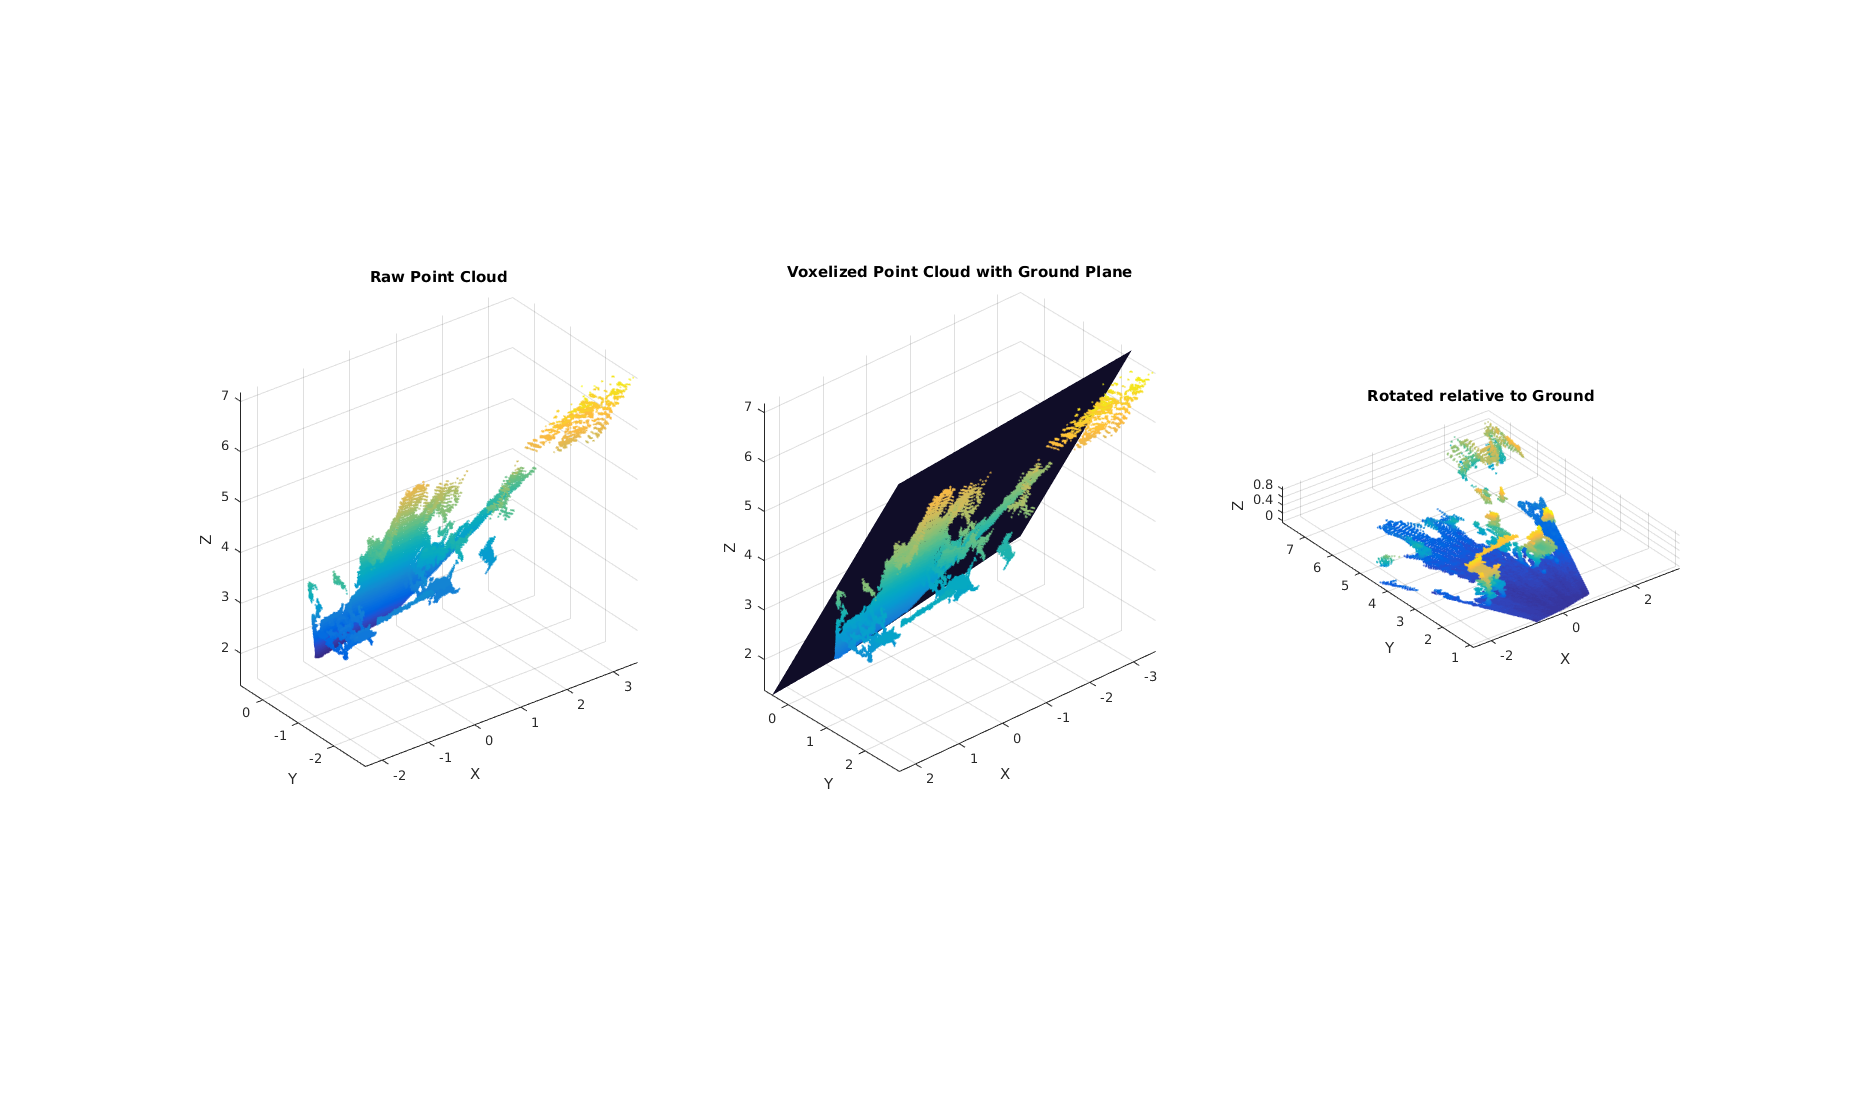
\includegraphics[width=6in]{figures/pointclouds.png}
\caption{Left: point cloud obtained from the RGBD sensor. Middle:
Downsampled point cloud with ground plane detected. Right: Rotated point cloud.}
\label{fig:pointclouds}
\end{figure}

% ====================
\subsection{Generating a 2D Map}
\label{sec:2dmap}
% ====================
We generate a 2D Map by projecting the 3D ground-aligned point cloud onto the
ground plane.
We classify each position on the 2D map as an object, the ground, or unknown.
Object and unknown classes are separated for use in
\autoref{sec:choosingparkingspot}.

Algorithm \autoref{alg:groundmapprojection} shows how the point cloud is
converted to a 2D map. It takes in the ground-aligned point cloud $P_{rotated}$
and two parameters: $gridStepSize$, a scalar in metres per pixel representing
the resolution of the map, and $groundThreshold$, the max height in metres that
a point can be considered part of the ground. This should be roughly the same
order of magnitude of $t$ from Algorithm \ref{alg:modifiedRansac}.

Let $p = (x_p, y_p, z_p) \in P_{rotated}$ be a of point in $\mathbb{R}^3$, with
$z_p$ representing the height above the ground for each point. Lines X to Y show
2D histograms are initialized to capture the location of ground and object
points. The histogram bounds are defined by taking the extremum points in both
the x and y dimensions.




A Gaussian blur with
a standard deviation of 0.7 is applied to filter out holes due to noise and
include a safety buffer. This is binarized on lines 12 and 13 by thresholding at
zero, resulting in a binary object map.
Similarly, the 2D ground histogram is binarized on lines 14 and 15 by first applying a Gaussian
blur with a standard deviation of 0.5 and thresholding at zero. 
Additionally, a 1m circle around the origin of the camera is assumed to be
viable positions in the ground map, which accounts for the minimimum range of
the RGBD camera. This is needed to ensure connectivity between the origin state
and farther feasible states, needed on line 2 in algorithm
\autoref{alg:feasibilitycheck}.

TODO talk about morphological dilation and erosion.

In a conservative fashion, any true pixels in the ground map that share a true
value in the object map is set to false, making the set of ground pixels and
object pixels mutually exclusive. 
% A third map is created for pixels that are not classified as a ground or object;
% hence each pixel must be classified as either on the ground plane, an object, or
% unknown.

\begin{algorithm}
\caption{TODO Ground Map Projection}
\label{alg:groundmapprojection}
\begin{algorithmic}[1]
\Require{$P_{rotated}$, $gridStepSize$, $groundThreshold$}
\Statex
\Function{GroundMapProjection}{$P_{rotated}, gridStepSize, groundThreshold$}
    \State $LB_x = \min_{p \in P_{rotated}}(x_p)$
    \State $UB_x = \max_{p \in P_{rotated}}(x_p)$
    \State $LB_y = \min_{p \in P_{rotated}}(y_p)$
    \State $UB_y = \max_{p \in P_{rotated}}(y_p)$
    \State $groundMap$, a 2D Histogram with bins spaced $gridStepSize$ metres apart
    \State $objectMap$, a 2D Histogram with bins spaced $gridStepSize$ metres apart
    \For{each point $p \in P_{rotated}$}
        \State $(x,y,z) \gets p$
        \If{$z < groundThreshold$}
            \State add $1$ to the appropriate $groundMap$ bin based on $(x,y)$
        \Else
            \State add $1$ to the appropriate $objectMap$ bin based on $(x,y)$
        \EndIf
    \EndFor
    \State $objectMap \gets GaussianBlur(objectMap, \sigma_1)$
    \State $objectMap \gets 1$ for each non-zero bin, $0$ otherwise

    \State $groundMap \gets GaussianBlur(groundMap, \sigma_2)$
    \State $groundMap \gets 0$ for each bin equal to zero and not already in $objectMap$, $1$ otherwise
\EndFunction
\Statex
\Ensure{$groundMap$, a 2D boolean array with values of $1$ representing the
ground, and $objectMap$}, a 2D boolean array with values of $1$ representing
impassible objects.
\end{algorithmic}
\end{algorithm}

\autoref{fig:groundobjectmap} shows an example of the resulting ground and
object map.

\begin{figure}
\centering
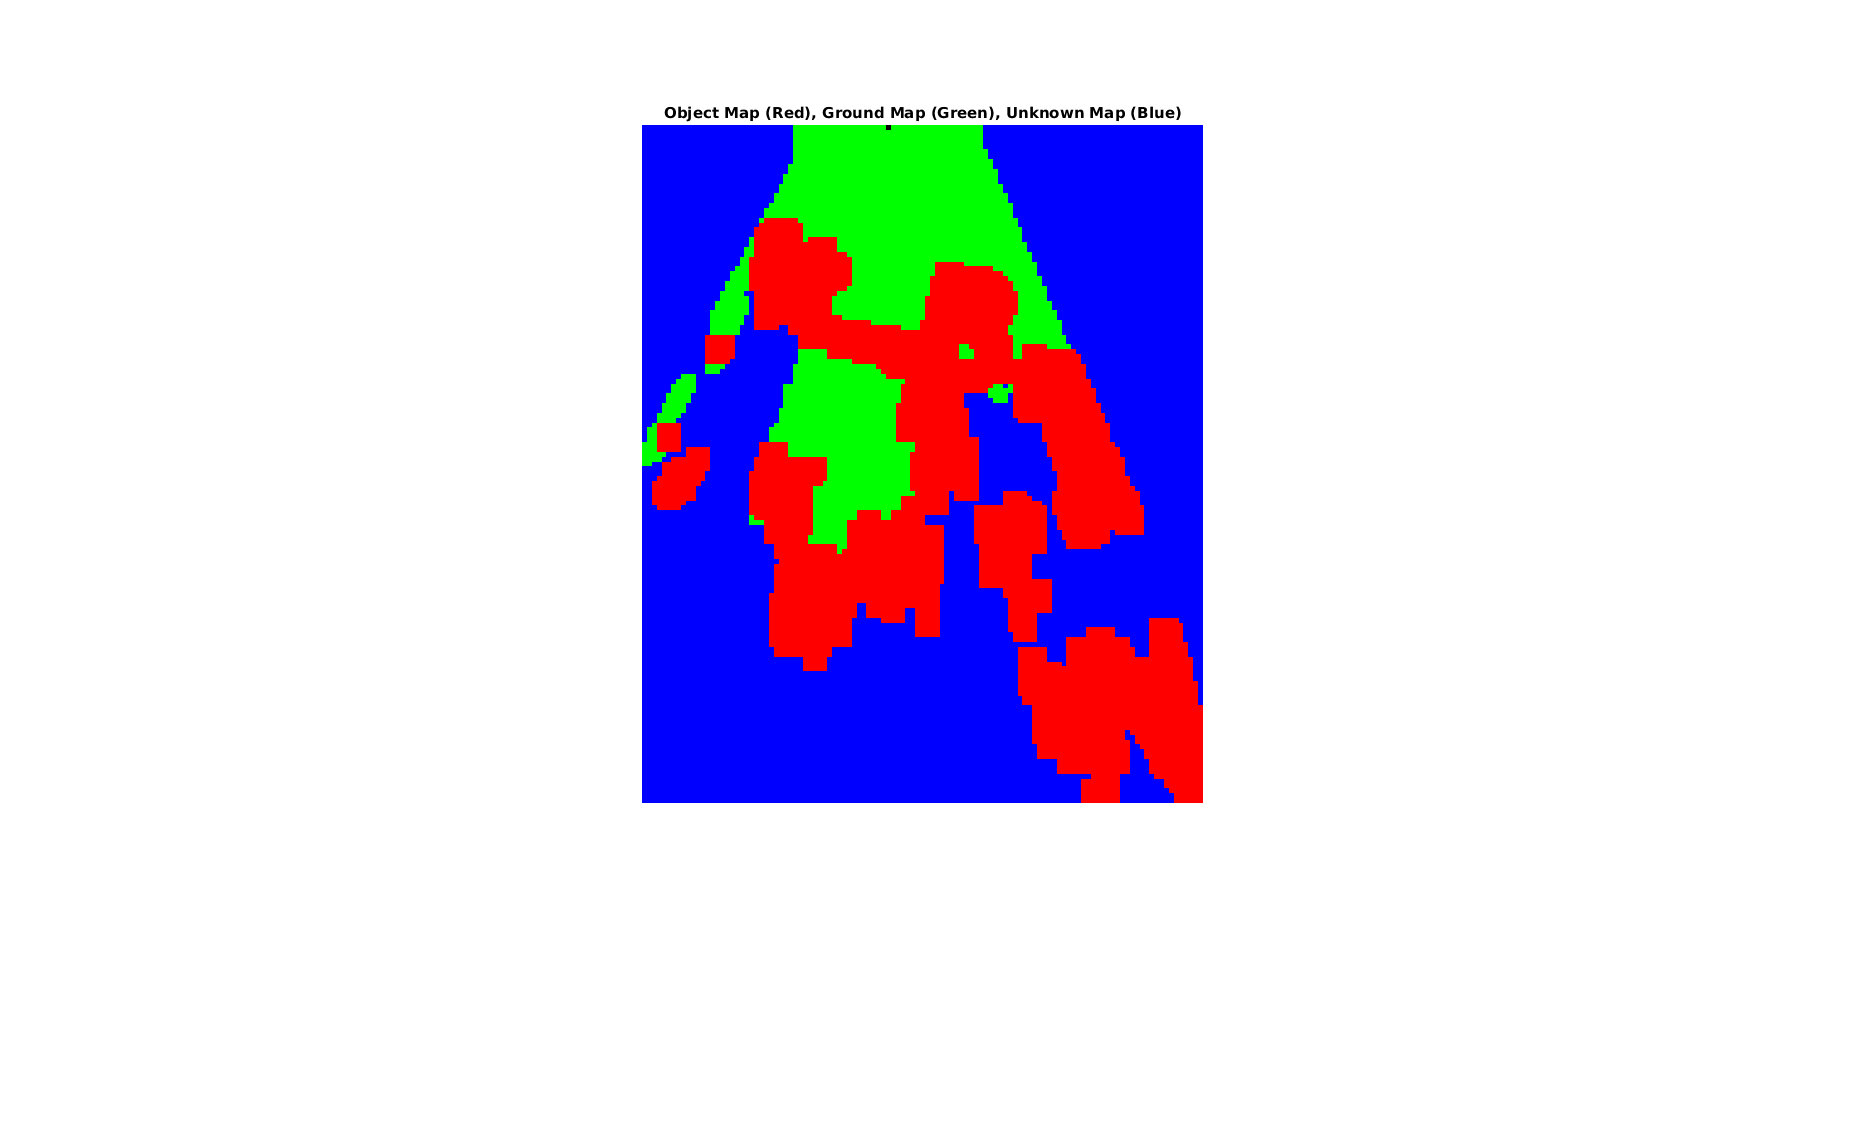
\includegraphics[width=5in]{figures/groundobjectmap.png}
\caption{2D projection of the point cloud. Green (light gray on black and white)
is classified as ground, red (medium gray) is classified as objects, and blue
(dark gray) is classified as unknown, determined by Algorithm
\autoref{alg:groundmapprojection}. The black pixel near the centre top
represents the location of the wheelchair during time of capture.}
\label{fig:groundobjectmap}
\end{figure}

% --------------------
\section{Motion Planning}
% --------------------

% --------------------
\subsection{Introduction to Motion Planning}
% --------------------
An in-depth introduction can be found in Chapter 1.3 of Lavalle
\cite{lavalle2006planning}.
% \begin{itemize}
% \item State
% \item Time
% \item Actions
% \item Initial and Goal States
% \item Feasibility and Optimality Criterion
% \item A Plan
% \end{itemize}

% --------------------
\subsection{Simple Motion Planning}
% --------------------
The simplest motion planning problems assume knowledge of a global map, a fixed
known goal state and a fixed known initial state. The problem is to determine a
feasible path from the initial state to the goal state. An optimality criterion
may also be applied to choose the best path if multiple feasible ones are found.

Notably, two important concepts are ignored in determining the path:
differential constraints of the system and the use of feedback. Differential
constraints refer to how states transition to other states, and is inherent in
real-world systems, eg. a system's dynamics. For example, a car can easily move
fowards and backwards, but cannot immediately move side to side, which may be
assumed when determining a path. Feedback refers to the technique of refining
further actions based on newly sensed data. In simulations feedback may not be
necessary, but in real-world systems, errors in sensing and modeling build up
over time without it.

In this simple case, the solution involves a generated path that is followed in
an open-loop manner, or if subject to real-world constraints (see
\autoref{fig:lavalle2006planning119}), the generated path is smoothed to obey
the system's dynamics and feedback is used to closely follow the path. "Notably
this approach is highly decoupled as feedback and dynamics are neglected in
constructing the original path" \cite{lavalle2006planning}. The smooth path may
now obey the robot's dynamics, but may no longer be feasible. Feedback is used
as an inefficient afterthought to stay on a track that itself may not be
feasible or optimal.

\begin{figure}
\centering
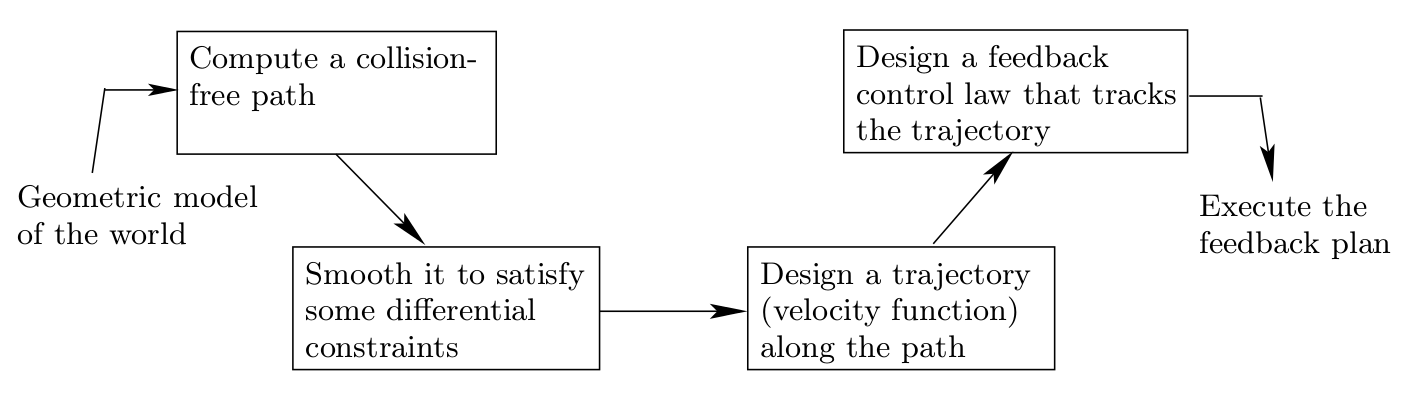
\includegraphics[width=3in]{figures/lavalle2006planning119.png}
\caption{From \cite{lavalle2006planning}. A refinement approach that has been
used for decades in robotics. Note the initial path is computed without
consideration of differential constraints or the use of feedback}
\label{fig:lavalle2006planning119}
\end{figure}

Even in this simple case, obtaining an optimal or even feasible path is not
straightforward if the state space is large. A* search for trivially sized state
spaces and sampling-based techniques such as RRTs (RRT* for optimality) and PRMs
have proven to be the methods of choice (citation?), though it is still an
ongoing field of interest (cite 2015 RRT/PRM papers).

The ROS Navigaiton Stack
(\url{http://www.dis.uniroma1.it/~nardi/Didattica/CAI/matdid/robot-programming-ROS-introduction-to-navigation.pdf})
is an example of this.
% --------------------
\subsection{Feedback Motion Planning}
% --------------------
Incorporating feedback directly when generating a path is a secondary option. 
For a full description of feedback motion planning, see Chapter 8 of Lavalle
\cite{lavalle2006planning}.
In the back-in parking problem, the trajectory to the goal state is assumed
visible, and hence generating a vector field may be suitable. A reliable model
and odometry data, however, varies from wheelchair to wheelchair, and so the
solution must be robust to model inaccuracies.

Two approaches can be taken: One, a target parking spot can be determined from
the initial position of the wheelchair, and the initial point cloud can be used
as a local map. The task is then to simultaneously localize the wheelchair's
position in the initial map while following a trajectory towards the parking
spot. This is visualized in \autoref{fig:determinedrive2}.
 
\begin{figure} % --------------------------------------
\centering
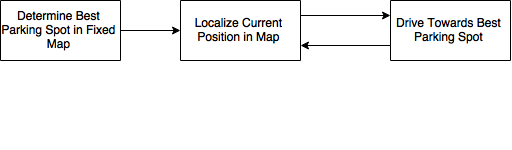
\includegraphics[width=3in]{figures/determinedrive2.png}
\caption{Feedback loop with a fixed goal state and map}
\label{fig:determinedrive2}
\end{figure}   % --------------------------------------

A second approach is to instead continuously update the initial map with new
sensor data, in effect performing SLAM on a constrained trajectory. The goal
state can then also be continously updated as new map information is ingested,
and the trajectory of the wheelchair will be updated based on this.
\autoref{fig:determinedrive1} illustrates this.
 
\begin{figure} % --------------------------------------
\centering
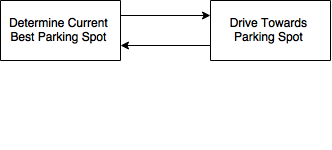
\includegraphics[width=3in]{figures/determinedrive1.png}
\caption{Feedback loop}
\label{fig:determinedrive1}
\end{figure}   % --------------------------------------

% ====================
\section{Related Work}
\label{sec:backinginlitreview}
% ====================
One way is to have a fixed, open-loop trajectory. This method is very old and
has been done for cars.

\cite{sermeno2006vision} uses vision-based PID control (page 17)

Angus's paper using PID

\subsection{Real-time Motion Planning}

From \cite{hauser2013recognition}:
Sampling-based motion planners such as Probabilistic Roadmaps (PRMs) and
Rapidly-Exploring Random Trees (RRTs) are effective at planning collision-free
motion for high-dimensional robot systems ( LaValle 2006), and have also been
successfully applied to hard real-time planing for 2D helicopters ( Frazzoli et
al. 2002) and ground vehicles ( Petti and Fraichard 2005). Recently they have
been applied to teleoperation interfaces for robot manipulator arms ( Hauser
2011). But these works have traditionally focused on finding feasible paths
rather than optimal ones.  Sampling-based approaches have been recently
developed for the optimal motion planning problem ( Karaman and Frazzoli 2010),
but they have not yet been applied to time- varying cost functions and moreover
converge too slowly for real-time use. An alternative approach is numerical
opti- mization over a trajectory parameterization ( Bobrow et al.  2001).
Optimization approaches can achieve optimality with a fast convergence rate,
albeit only locally. Our hybrid plan- ner combines the strength of
sampling-based and numeri- cal approaches and is designed specifically to
produce high- quality paths quickly for a broad class of cost functions.

% ====================
\section{Visual Odometry}
% ====================
Pictures of sequences

% ====================
\section{Pure Pursuit Path Planner}
% ====================

% ====================
\section{Results}
% ====================
Qualtitative Pictures.

Time to reach.

% 
% % --------------------
% \section{Practical Options}
% % --------------------
% 
% \begin{figure}
% \centering
% 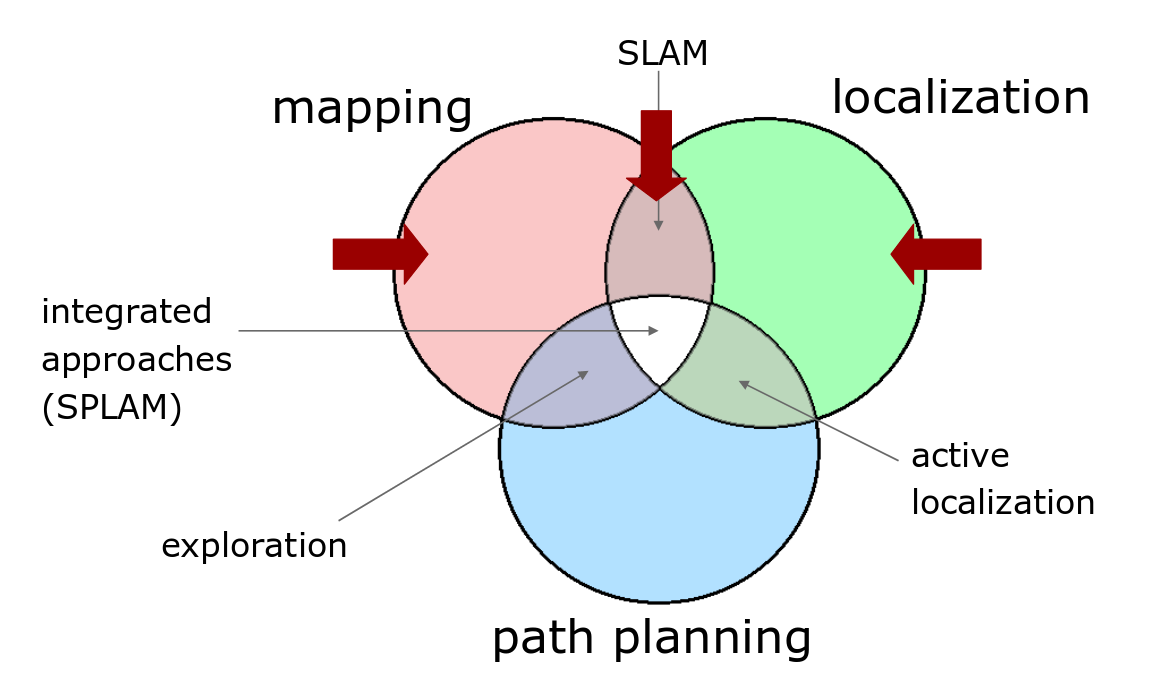
\includegraphics[width=3in]{figures/mappinglocalizationpathplanningvenndiagram.png}
% \caption{Venn Diagram of Localization, Mapping and Path Planning}
% \label{fig:mappinglocalizationpathplanningvenndiagram}
% \end{figure}
